%%%%%%%%%%%%%%%%%%%%%%%%%%%%%%%%%%%%%%%%%%%%%%%%%%%%%%%%%%%%%%%%%%
%%%%%%%% ICML 2017 EXAMPLE LATEX SUBMISSION FILE %%%%%%%%%%%%%%%%%
%%%%%%%%%%%%%%%%%%%%%%%%%%%%%%%%%%%%%%%%%%%%%%%%%%%%%%%%%%%%%%%%%%

% Use the following line _only_ if you're still using LaTeX 2.09.
%\documentstyle[icml2017,epsf,natbib]{article}
% If you rely on Latex2e packages, like most moden people use this:
\documentclass{article}

% use Times
\usepackage{times}
% For figures
\usepackage{graphicx} % more modern
%\usepackage{epsfig} % less modern
\usepackage{subfigure} 

% For citations
\usepackage{natbib}

% For algorithms
\usepackage{algorithm}
\usepackage{algorithmic}

% As of 2011, we use the hyperref package to produce hyperlinks in the
% resulting PDF.  If this breaks your system, please commend out the
% following usepackage line and replace \usepackage{icml2017} with
% \usepackage[nohyperref]{icml2017} above.
\usepackage{hyperref}

% Packages hyperref and algorithmic misbehave sometimes.  We can fix
% this with the following command.
\newcommand{\theHalgorithm}{\arabic{algorithm}}

% Employ the following version of the ``usepackage'' statement for
% submitting the draft version of the paper for review.  This will set
% the note in the first column to ``Under review.  Do not distribute.''
\usepackage{icml2017} 

% Employ this version of the ``usepackage'' statement after the paper has
% been accepted, when creating the final version.  This will set the
% note in the first column to ``Proceedings of the...''
%\usepackage[accepted]{icml2017}


% The \icmltitle you define below is probably too long as a header.
% Therefore, a short form for the running title is supplied here:
\icmltitlerunning{Dimensionality Reduction using Dictionary Learning and Visualization using Manifold learning}

\begin{document} 

\twocolumn[
\icmltitle{Dimensionality Reduction using Dictionary Learning and Visualization using Manifold learning}

% It is OKAY to include author information, even for blind
% submissions: the style file will automatically remove it for you
% unless you've provided the [accepted] option to the icml2017
% package.

% list of affiliations. the first argument should be a (short)
% identifier you will use later to specify author affiliations
% Academic affiliations should list Department, University, City, Region, Country
% Industry affiliations should list Company, City, Region, Country

% you can specify symbols, otherwise they are numbered in order
% ideally, you should not use this facility. affiliations will be numbered
% in order of appearance and this is the preferred way.
\icmlsetsymbol{equal}{*}

\begin{icmlauthorlist}
\icmlauthor{Aeiau Zzzz}{equal,to}
\icmlauthor{Bauiu C.~Yyyy}{equal,to,goo}
\icmlauthor{Cieua Vvvvv}{goo}
\icmlauthor{Iaesut Saoeu}{ed}
\icmlauthor{Fiuea Rrrr}{to}
\icmlauthor{Tateu H.~Yasehe}{ed,to,goo} 
\icmlauthor{Aaoeu Iasoh}{goo}
\icmlauthor{Buiui Eueu}{ed}
\icmlauthor{Aeuia Zzzz}{ed}
\icmlauthor{Bieea C.~Yyyy}{to,goo}
\icmlauthor{Teoau Xxxx}{ed}
\icmlauthor{Eee Pppp}{ed}
\end{icmlauthorlist}

\icmlaffiliation{to}{University of Torontoland, Torontoland, Canada}
\icmlaffiliation{goo}{Googol ShallowMind, New London, Michigan, USA}
\icmlaffiliation{ed}{University of Edenborrow, Edenborrow, United Kingdom}

\icmlcorrespondingauthor{Cieua Vvvvv}{c.vvvvv@googol.com}
\icmlcorrespondingauthor{Eee Pppp}{ep@eden.co.uk}

% You may provide any keywords that you 
% find helpful for describing your paper; these are used to populate 
% the "keywords" metadata in the PDF but will not be shown in the document
\icmlkeywords{boring formatting information, machine learning, ICML}

\vskip 0.3in
]

% this must go after the closing bracket ] following \twocolumn[ ...

% This command actually creates the footnote in the first column
% listing the affiliations and the copyright notice.
% The command takes one argument, which is text to display at the start of the footnote.
% The \icmlEqualContribution command is standard text for equal contribution.
% Remove it (just {}) if you do not need this facility.

%\printAffiliationsAndNotice{}  % leave blank if no need to mention equal contribution
\printAffiliationsAndNotice{\icmlEqualContribution} % otherwise use the standard text.
%\footnotetext{hi}

\begin{abstract} 
Dictionary Learning is a representational learning method of writing the input data as a Linear combination of elements such that the code is sparse which relaxes the condition that components can be non orthogonal. Dictionary learning is very useful specifically for image analysis. It is generally used in applications like De-noising, In-painting, De-mosaicking, Video processing etc. Dictionary learning can also be made to restrict to convert the data into low dimensional space and hence can be used in dimensionality reduction. We wish to analyze different ways to do dimensionality reduction using various techniques and later visualize them using Manifold Learning.
\end{abstract} 

\section{Introduction}
\label{introduction}

In Machine Learning, in many algorithms, the speed is greatly hindered with large number of features. Many features don't add a lot of information and hence can be ignored within certain limit. Dimensionality reduction is the technique used to do the aforementioned task. Several algorithms like PCA, Manifold Learning etc can be used for Dimensionality reduction.The main advantage of using Dimensionality reduction is increased speed. Also since we remove the noise, the accuracy also increases in many cases. Dictionary Learning is another algorithm which can be used for dimensionality reduction.  Sparse Dictionary Learning expresses the input signal as a sparse Linear combination of Dictionary elements. The Sparsity can be encoded in several different ways and we want to experiment with different ways of encoding sparsity and how they influence the speed, accuracy of classifiers on classification problem. The paper is organized as follow. Section 2 talks about different approaches of dictionary learning, Section 3 talks about Visualizing the Dictionary Learning's output using Manifold Learning. Section 4 discusses results of various classifiers and work on other datasets. Section 5 has a discourse of future extensions and other attempts to learn the process better and limitations of our dictionary learning.


\section{Dictionary Learning}
Basic problem of Dictionary Learning\cite{mairal2009online} is given a dataset $X = [x_{1},x_{2},.....,x_k], x_i \in \mathcal{R}^d$ we wish to express it as $D*W$ where $D \in \mathcal{R}^{d x n}$ is the dictionary or the basis and $W \in \mathcal{R}^{n x k} $ where the vectors is R represent the contribution/representation of each component of dictionary. Now encode sparsity we specify the optimization problem as \[ argmin_{D,W} ||X - DW||_2^2 + ||W||_{.} \] Where $|| ||_{.}$ is a sparse norm. When $n>d$ we call the problem as overcomplete problem and when $n<d$ we call the problem as an undercomplete problem. For dimensionality reduction we will be using the latter one. The main advantage of using dictionary learning is unlike PCA we don't need to specify orthogonality as a constraint. This is mainly useful is classification tasks. To test the power of Dictionary learning we used MNIST dataset\cite{lecun2010mnist} as a reference and used KNN classifier as the basis of accuracy.% Head 2
\subsection{L0 norm}
Since true sparsity is represented by the L0 norm we tried to optimize the L0 norm problem of Dictionary Learning to reduce the dimensions. The number of dimensions we choose were 100. We used sklearn\cite{pedregosa2011scikit} library to solve this problem. Since L0 norm problem is non-convex, we used the Orthogonal Matching Pursuits(OMP) Algorithm. We observed that we get an error rate of about 4.2 \% with the 100 dimensional space in about 500 iterations. We also noted that KNN classifier's accuracy with the original MNIST dataset is 5\% so we get a better accuracy with the new dimensional space. Also ,run time complexity of KNN is O(d), we made the algorithm about 8 times faster for a better accuracy rate. However PCA gave an accuracy of 2.7\% and solving PCA is much faster problem. So even though our problem is good, we needed improvements in speed and accuracy to make it useful.
\begin{figure}[ht]
\vskip 0.2in
\begin{center}
\centerline{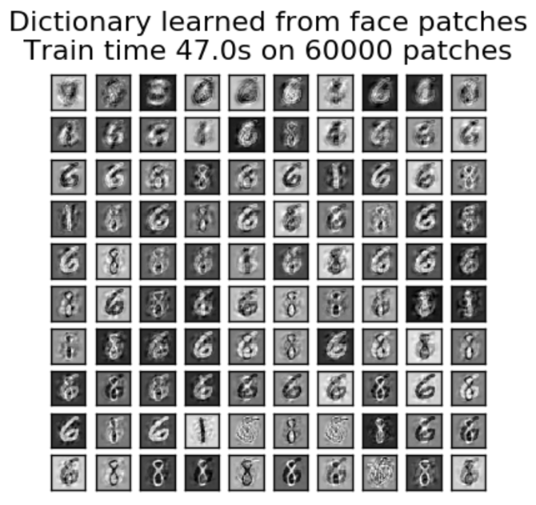
\includegraphics[width=50mm,scale=1.0]{Dictionary.PNG}}
\caption{MNSIT data representation through Dictionary Learning}
\label{icml-historical}
\end{center}
\vskip -0.4in
\end{figure} 

% Head 3
\subsection{L1 norm}
Since we needed to increase the speed of computation it would be easier if we can solve a convex optimization problem. So we tried using L1 norm as sparsity measure to optimize the problem. Now we used Lasso and Lars optimizers to solve the problems. Even though we observed slight increase in speed, the objective was still converging after 500 iterations. So instead we used FISTA\cite{beck2009fast} to make it converge in 300 iterations. We observed that when we go to 500 iterations FISTA gives a slightly better error rate of 3.87\%.
 
\subsubsection{FISTA}
Since FISTA has a higher convergence rate, we used the algorithm(Algorithm 1) on MNIST data. 
\begin{algorithm}[ht]
   \caption{FISTA}
   \label{alg:example}
\begin{algorithmic}
   \STATE {\bfseries Input:} W, b, $\lambda$, maxIter
   \STATE x=Array of shape W.columns X b.columns
   \STATE obj = []
   \STATE $t=1$
   \STATE z = copy(x)
   \STATE $L = ||W||_{2}^{2}$
   \STATE $t_{old} = time()$
   \FOR{$i=1$ {\bfseries to} $maxIter$}
      \STATE $x_{old} = copy(x)$
      \STATE $z = z + W^{T}(b-Wz)$
      \STATE $x = SOFT-THRESHOLDING(z, \lambda/L)$
      \STATE $t_{new} = t$
      \STATE $t = (1. + \sqrt{1. + 4.0*t^{2}})/2$
      \STATE $z = x + ((t_{old}-1.)/t * (x-x_{old}))$
      \STATE $obj_{new} = 0.5 * ||Wx-b||_{2}^{2} + \lambda ||W||$
      \STATE $obj.add((time - t_{0}, obj_{new}))$
   \ENDFOR
   \end{algorithmic}
\end{algorithm}


\subsection{Other sub-optimal Norms}
We also tried Nuclear norm as we wanted to penalize W if it had higher dimensions. We observed a slightly better error rate of 3.57\%. W also tried to put an L2 regularization on dictionary to avoid overfitting and got an accuracy of 3.67\%.

\subsection{Best Solution}
The best solution we found out was using an Elastic Net\cite{zhou2011manifold} instead of solving the Lasso problem on W. This means that W instead of D was being overfit. We got an error rate of 2.97\% which is fairly close to that of PCA. Combined with FISTA it converges even faster. Hence we have solved both the problems of Speed and accuracy using this approach

\section{Manifold Learning}

Manifold learning\cite{gu2006improved} is a technique for non-linear dimensionality reduction, as opposed to PCA, which is a linear dimensionality reduction. It helps in visualising data which might have many dimensions, by trying to find the lower dimensional manifold which is present in the higher dimensional data.

After comparing the Isometric Mapping, Locally Linear Embedding and t-SNE, we found that the best results are obtained from t-SNE.
\begin{figure}
    \centering
    \begin{minipage}{0.45\textwidth}
        \centering
        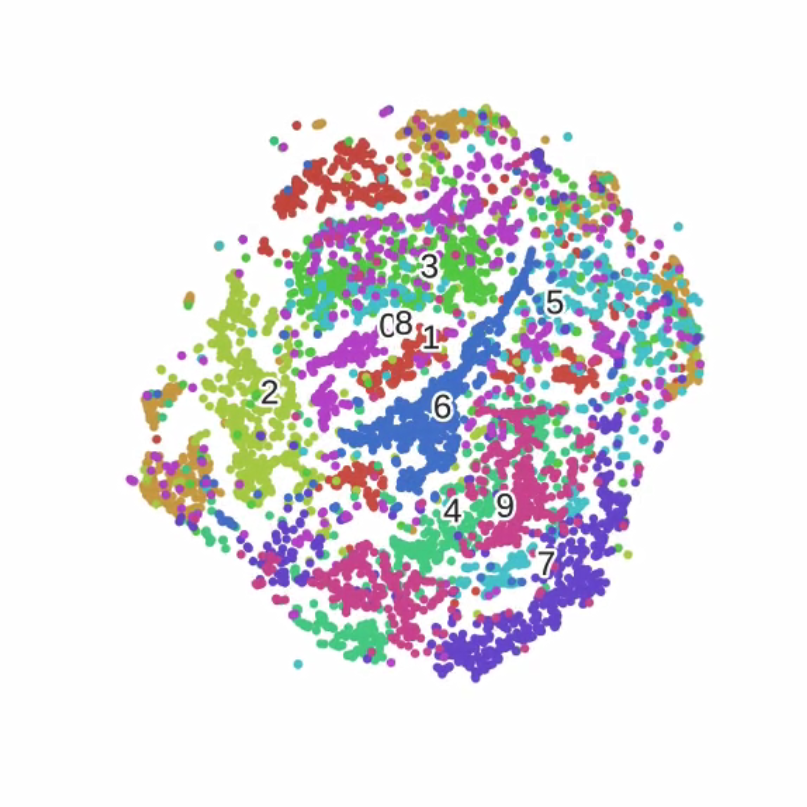
\includegraphics[width=0.8\textwidth]{MNIST_10.png} % first figure itself
        \caption{Manifold Learning on 10\% MNIST data}
    \end{minipage}\hfill
    \begin{minipage}{0.45\textwidth}
        \centering
        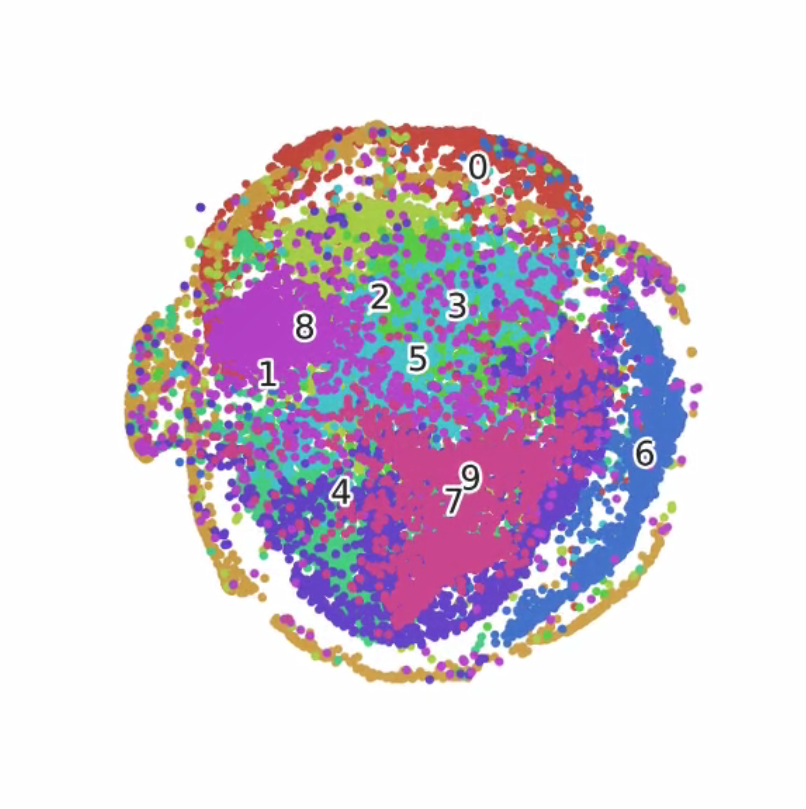
\includegraphics[width=0.8\textwidth]{MNIST_30.png} % second figure itself
        \caption{Manifold Learning on 30\% MNIST data}
    \end{minipage}
\end{figure}

\subsection{t-SNE}

t-distributed Stochastic Neighbor Embedding(t-SNE)\cite{maaten2008visualizing} converts the similarity of the data to probabilities. It's computationally intensive, and takes the most time compared to the other embedding models. It tries to learn the joint probability distribution of the data distribution in the higher dimensional space and then tries to replicate that in the low dimensional space by optimizing the KL divergence using Stochastic Gradient.

We learned how the clusters get formed in the final output of t-SNE by making a GIF of the training process. To do this, we had to patch the gradient descent method of tsne in scikit library, by adding code which could save the intermediate positions of the points, which was later converted into a GIF.

It was interesting to note that t-SNE has overlapping clusters of digits that actually look a little similar, like 4 and 9, and 0 and 8. Digits which don't look similar are as expected quite far apart from each other in the t-SNE result.

\section{Results and Interpretation}
The results obtained by using various classifiers are captured in the following table:\\
\begin{tabular}{ |p{4cm}|p{2cm}|  }
	\multicolumn{2}{}{} \\
	\hline
	Classifier & Error\\
	\hline
	KNN  &  4.1 \% \\
	Linear SVM  & 14.81 \% \\
	Gaussian Naive Bayes & 16.88 \%\\
	Multi-Layer Perceptron  & 7.95 \%\\
	\hline
\end{tabular}
\vspace{0.1in}
\\
We can compare the results we have obtained with the state of the art error rates obtained on these classifiers without using sparse coding. On the basis of the results, we can infer that the neighborhood property of the data points in being maintained as the KNN error was very low. The Gaussian Naive Bayes Classifier also gave about the same error, which indicates that the distribution of the data is also being preserved. However, we get a higher error rate for the Linear SVM classifier, which suggests that the linearity of the data is not being maintained. 

\section{Future Work}

We want to work on making dictionary learning invariant to affine transformations. On the AffNist dataset, which is MNIST data on which various affine transformations have been applied, our error rate is 30\%, but this can be reduced using hierarchical dictionary learning.
We plan to apply the manifold learning algorithms on a more challenging dataset like the CIFAR-10 image dataset. It will be interesting to see which of the embedding models works best with that dataset.
We have applied TSNE-visualization on the sparse coded vectors returned after dictionary learning. It will be interesting to compare these manifolds with the ones created on the normal dataset.

\section{Conclusion}
One of the observations is that Orthogonality of components is important for dimensionality reduction as PCA does better in most cases. However we see that with enough tuning parameters and change in Objective functions we can make dictionary learning perform better.

We observed that the clusters formed by t-SNE become less and less clear as the we include more points from the dataset. We think this happens because as we add more data, we're adding more noise to the dataset as well, thereby reducing the distance between various digits in the lower dimensions.

\section*{Acknowledgements}

The authors would like to thank Dr. Lior Horesh and Dr. Julie Novak for providing insightful suggestions about the project, especially the suggestion to learn the manifold that the data lives upon and to make our dictionary learning process invariant to affine transformations.

The work is presented as a part of the final project for the course COMS 4772: Advanced Machine Learning in the Spring semester of 2017.

%Sets the bibliography style to UNSRT and imports the 
%bibliography file "samples.bib".
\bibliography{bibliography}
\bibliographystyle{icml2017}
\end{document} 


% This document was modified from the file originally made available by
% Pat Langley and Andrea Danyluk for ICML-2K. This version was
% created by Lise Getoor and Tobias Scheffer, it was slightly modified  
% from the 2010 version by Thorsten Joachims & Johannes Fuernkranz, 
% slightly modified from the 2009 version by Kiri Wagstaff and 
% Sam Roweis's 2008 version, which is slightly modified from 
% Prasad Tadepalli's 2007 version which is a lightly 
% changed version of the previous year's version by Andrew Moore, 
% which was in turn edited from those of Kristian Kersting and 
% Codrina Lauth. Alex Smola contributed to the algorithmic style files.  
